% Chapter Template

\chapter{Introducción al magnetismo superficial} % Main chapter title

\label{Chapter5} % Change X to a consecutive number; for referencing this chapter elsewhere, use \ref{ChapterX}


%----------------------------------------------------------------------------------------

%----------------------------------------------------------------------------------------
%	SECTION 1
%----------------------------------------------------------------------------------------

\section{Caracterización de propiedades y defectos por Técnicas Magnéticas Superficiales}

Los campos magnéticos próximos a las superficies de separación entre medios experimentan una suave transición entre las condiciones de frontera  y los campos impuestos macroscópicamente por la magnetización dominante en volumen. En particular nos interesarán los campos en el aire cercanos a las superficies de sólidos que puedan tener o no corrientes superficiales.


\section{Frontera magnética.}

El campo magnético exterior próximo a la superficie de los sólidos es afectado tanto por las condiciones de frontera entre el medio y el sólido como por la presencia de anomalías en el seno de material. Las dos propiedades más relevantes serán $\mu$ y $\sigma_{e}$ (la permeabilidad magnética y la conductividad eléctrica) las que nos permitirán clasificar los materiales en tres grupos según sean:

\begin{itemize}
	\item Materiales del grupo ferro, ferri y para - magnéticos (ffp $\mu_{r}>1$). 	
	\item Materiales no ffp, conductores ($\sigma_{e}>0$).
	\item Materiales no ffp, no conductores ($\sigma_{e}=0$).	
\end{itemize}


Deberemos tener siempre en cuenta las condiciones de frontera del electromagnetismo clásico entre dos medios 1 y 2:

Ley de Ampere:
\begin{equation}
\begin{aligned}
	&\hat{n}_{1,2} \times(\overrightarrow{H_{1}}-\overrightarrow{H_{2}})  = \overrightarrow{k_{e}} \quad \text{con}  \quad	\\
	&\overrightarrow{k_{e}}=\lim_{h\rightarrow 0} 	\left(\overrightarrow{J_{e}}+\dfrac{\partial \overrightarrow{D}}{\partial t} \right) h \left[ \dfrac{A}{m}\right] 
\end{aligned}
\end{equation}

Ley de Faraday:
\begin{equation}
\begin{aligned}
	& \hat{n}_{1,2} \times(\overrightarrow{E_{1}}-\overrightarrow{E_{2}}) = -\overrightarrow{k_{m}} \quad \text{con}  \quad	\\
	&\overrightarrow{k_{m}}=\lim_{h\rightarrow 0} 	\left(\overrightarrow{J_{m}}+\dfrac{\partial \overrightarrow{B}}{\partial t} \right) h \left[ \dfrac{V}{m}\right] 
\end{aligned}
\end{equation}

Ley de Gauss eléctrica:
\begin{equation}
\begin{aligned}
	& \hat{n}_{1,2} \cdot (\overrightarrow{D_{1}}-\overrightarrow{D_{2}}) = -\overrightarrow{\sigma_{e}} \quad \text{con}  \quad	\\
	&\sigma_{e}=\lim_{ds\rightarrow 0} 	\left(\rho_{e}+\dfrac{\partial \overrightarrow{B}}{\partial t} \right) ds \left[ \dfrac{As}{m}\right] 
\end{aligned}
\end{equation}

Ley de Gauss magnética: 
\begin{equation}
\begin{aligned}
	& \hat{n}_{1,2} \cdot (\overrightarrow{B_{1}}-\overrightarrow{B_{2}}) = -\overrightarrow{\sigma_{m}} \quad \text{con}  \quad	\\
	&\sigma_{m}=\lim_{ds\rightarrow 0} 	\left(\rho_{m}+\dfrac{\partial \overrightarrow{B}}{\partial t} \right) ds \left[ \dfrac{Vs}{m}\right] 
\end{aligned}
\end{equation}

Siendo $\hat{n}_{1,2}$ el versor normal a la superficie que apunta de $1 \rightarrow 2$. También  observemos que las condiciones de frontera puntuales se calculan encerrando las circulaciones o los volúmenes hasta hacerlos tender a 0.

En la ley de Gauss para el campo magnético apelamos al concepto de cargas magnéticas, a sabiendas de que es un artificio solo válido para la representación de campos magnéticos en el exterior de los volúmenes, 

Suponiendo medios \textbf{lineales isótropos y homogéneos (LIH)} tendremos que para cada medio se cumplirá que:

\begin{equation}
	\overrightarrow{B}=\mu \overrightarrow{H} \quad \text{y} \quad \overrightarrow{D}= \epsilon \overrightarrow{E}
\end{equation}

Limitándonos al campo magnético tendremos que las ecuaciones de frontera adoptan la forma:

\begin{equation}
	\label{eq:50}
	\dfrac{B_{t1}}{\mu_{1}} -\dfrac{B_{t2}}{\mu_{2}} =k_{et} \quad \text{y} \quad B_{n1}-B_{n2} =  \sigma_{m} 
\end{equation}

Donde los subíndices $t$ y $n$ se refieren a las direcciones normal y tangente a la superficie, con $k_{et}$ la densidad de corriente superficial en la dirección tangente y $\sigma_{m}$ será la densidad monopolar magnética equivalente.

En ausencia de corrientes superficiales, la ecuación \ref{eq:50} se convertirá en:

\begin{equation}
	\label{eq:51}
	\dfrac{B_{t1}}{\mu_{1}} -\dfrac{B_{t2}}{\mu_{2}} \rightarrow \left( \dfrac{\mu_{2}}{\mu_{1}}\right)  B_{t1}= B_{t2}
\end{equation}

Que es el resultado ya conocido que nos dice que en un medio con $\mu_{2}\gg\mu_{1}$ las líneas de campo magnético tangente tenderán a curvarse hacia la superficie del material de mayor $\mu$ y a aumentar su intensidad proporcionalmente.

La presencia de corrientes superficiales $k_{et}$ cambiaría la expresión según:

\begin{equation}
	\label{eq:52}
	\dfrac{B_{t1}}{\mu_{1}} - k_{et} = \dfrac{B_{t2}}{\mu_{2}} \rightarrow \left( \dfrac{\mu_{2}}{\mu_{1}}\right) B_{t1} - \mu_{2} k_{et} = B_{t2}
\end{equation}

Si suponemos $B_{t1}$ despreciable en el primer medio la expresión anterior se transforma en:

\begin{equation}
	\label{eq:53}
	 - \mu_{2} k_{et} = B_{t2}
\end{equation}

Expresión que nos dice que todo el campo tangente en el segundo medio es producto de las corrientes superficiales.

\subsection{Sólidos Ferromagnéticos}

Los sólidos ferromagnéticos en presencia del campo magnético terrestre presentan una magnetización inducida, fuertemente condicionada por las condiciones de frontera magnética. El campo inducido por el campo magnético terrestre divergirá en las zonas de discontinuidad superficial del material y en zonas de stress, oquedades y oclusiones de otros materiales en el seno del material original. Para estos sólidos es particularmente útil el Método de la Memoria Magnética. El método también puede aplicarse, con menor grado de facilidad, a materiales paramagnéticos y ferrimagnéticos.

\subsubsection{Método de la Memoria Magnética (MMM)}

El científico Ruso Anatoli Dubob desarrolló el MMM basado en la detección y medición del campo de fuga magnética propio del material (Surface Magnetic Leakeage field o SMLF), que surge en las zonas de acumulaciones de luxaciones de alta densidad de materiales ferromagnéticos y paramagnéticos. La histéresis de las magnetodislocaciones es un efecto subyacente de la memoria magnética de metal y tiene lugar durante la fabricación de productos en la formación de tensiones internas y en su funcionamiento bajo acción de cargas de trabajo. 

Cuando un sólido ferromagnético se enfría por debajo de su temperatura de Curie, el campo magnético terrestre genera un patrón de dominios. Asociados a procesos de térmicos o por deformación en frío se producen defectos en la estructura policristalina. Algunos defectos estructurales presentan concentraciones de esfuerzos y deformaciones importantes. Estas concentraciones alteran localmente los dominios magnéticos y producen, a su vez, heterogeneidades en la magnetización que pueden ser detectadas utilizando la dispersión del campo magnético en la superficie de los cuerpos. La medición de las no uniformidades de la magnetización permite detectar esos defectos en forma no destructiva. 

En general no es posible obtener información en forma global del campo magnético autogenerado en sólidos. La información se forma y se puede obtener solo en pequeñas regiones donde los defectos tiene una influencia significativa por su cercanía y no se ven afectados por otros defectos. Es de esperarse que en los defectos significativos, el campo externo de la tierra no haya podido ejercer una influencia marcada si la energía asociada a la producción del defecto es muy superior a la aportada por el campo magnético externo.

El método \textbf{MMM} se aplica para la solución de problemas del tipo de:


\begin{itemize}
	\item Control de calidad al 100\% de los productos de piezas de construcción de máquinas y control de heterogeneidad del metal.
	
	\item Control de calidad de juntas de soldadura (Aquí la soldadura es parte de un complejo sistema de factores vinculando la: heterogeneidad estructural-mecánica, lo defectos de soldadura y las concentraciones de estrés estructural.
	
	\item Diagnóstico temprano de daños por fatiga del metal, Estimación y pronóstico del tiempo de vida media de un equipo.
	
\end{itemize}

El \textbf{MMM} se puede aplicar tanto en sólidos bajo carga (en tensión como en el caso de piezas de maquinaria) así como después del retiro de las cargas, cuando la pieza no se encuentra solicitada. El perfil magnético formada bajo la acción de las cargas de trabajo queda parcialmente congelado después de la descarga en virtud de la "histéresis de dislocación magnética". Esto la posibilidad de evaluar el estado real de tensiones de la pieza y revelar en etapas tempranas las zonas de daño máximo al leer los campos utilizando dispositivos de medición de campo especiales. Es importante destacar que los dispositivos de medición de campos magnéticos no tienen una norma mundial por lo que cada instrumento presenta características y singularidades únicas y las mediciones no suelen ser referidas a un patrón sino que son relativas entre sí desde un estado base.

\begin{figure}[h]
	\centering
	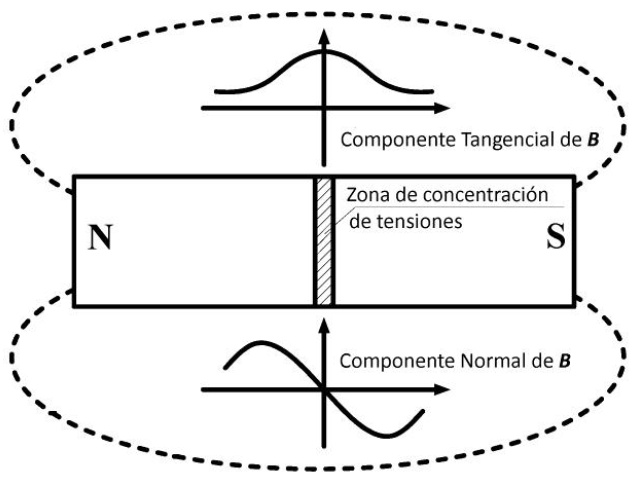
\includegraphics[width=0.75\textwidth]{./Figures/fig50}
	\caption{Campos magnéticos superficiales en presencia de zona de concentración de tensiones.}
	\label{fig:50}
\end{figure}. 


\subsection{Región de Influencia Magnética de un Defecto}

Se conoce experimentalmente \citep{Lauer:1} que la magnetización local se puede ver afectada por la presencia de inclusiones no ferromagnéticas o cavidades que poseen permeabilidades mucho menores que la del material ferromagnético adyacente, generando heterogeneidades magnéticas primarias que dispersan las líneas del flujo. También es sabido \citep{Lauer:1} que la magnetización natural de una pieza ferromagnética se modifica con la aplicación de cargas externas y con las concentraciones de tensiones mecánicas asociadas a defectos presentes en el material (aglomeraciones de dislocaciones, micro-poros, micro-fisuras, inclusiones, cavidades, fisuras). Estas perturbaciones localizadas de la magnetización natural son una manifestación del efecto magneto-elástico \citep{MagnetoElastic}. Como tales, originan heterogeneidades magnéticas secundarias de suma importancia desde el punto de vista del ensayo no destructivo mediante el MMM. A cada defecto significativo único o defecto equivalente obtenido por combinación de defectos próximos, se le puede asociar una región $\mathit{\mathbf{R}}_{mag}$ que puede considerarse como la región de influencia magnética del defecto. Esta región comprende todos los puntos en los cuales es significativa la perturbación en la magnetización producida por el defecto en cuestión. La perturbación se manifiesta en un cambio de dirección en las líneas de flujo de la inducción $\vec{\mathit{\mathbf{B}}}$ y en una variación en su magnitud. Si el defecto dispersa las
líneas estas saldrán o entrarán del sólido a través de la frontera más próxima como se puede ver en la figura \ref{fig:51}.

\begin{figure}[h]
	\centering
	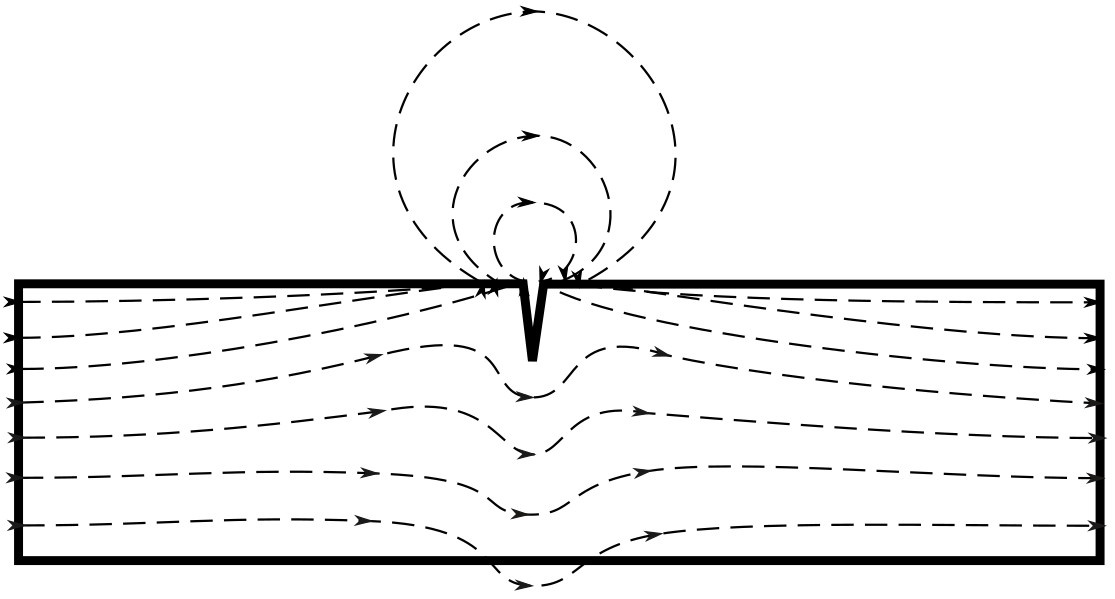
\includegraphics[width=0.8\textwidth]{./Figures/fig51}
	\caption{Fuga de líneas de flujo magnético asociada a grietas y discontinuidades en la superficie del material.}
	\label{fig:51}
\end{figure}. 

En la figura \ref{fig:51} vemos el perfil de los campos magnéticos asociados a perturbaciones en el medio debidas a heterogeneidades magnéticas primarias.

Si la fuga de flujo hacia (o desde) el aire es lo bastante significativa, puede medirse el campo de fuga (auto-campo de fuga en la jerga del MMM) utilizando sensores de campo magnético situados lo bastante próximos a la frontera.


En el caso general tendremos una combinación de condiciones de campos debido a tensiones, grietas y otros factores combinados.


El ensayo de álabes de turbina son una aplicación frecuente del MMM. En la figura \ref{fig:52} observamos la presencia de fisuras a lo largo de la misma.

\begin{figure}[H]
    \centering
    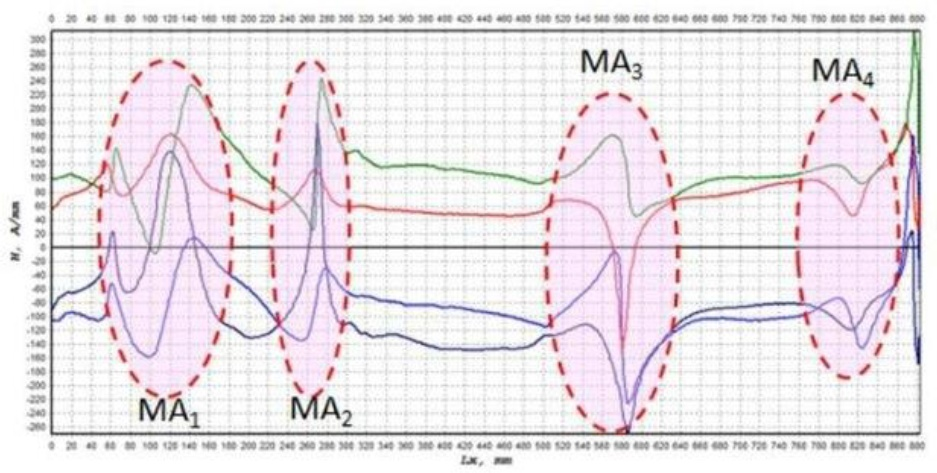
\includegraphics[width=0.8\textwidth]{./Figures/fig52}
	\caption{$MA_{1}-MA_{4}$ fisuras en álabes a lo largo sobre y sobre el plano}
	\label{fig:52}
\end{figure}

En la figura \ref{fig:53} vemos el mismo mismo ensayo del alabe pero medidos los campos sobre el canto.

\begin{figure}[H]
    \centering
    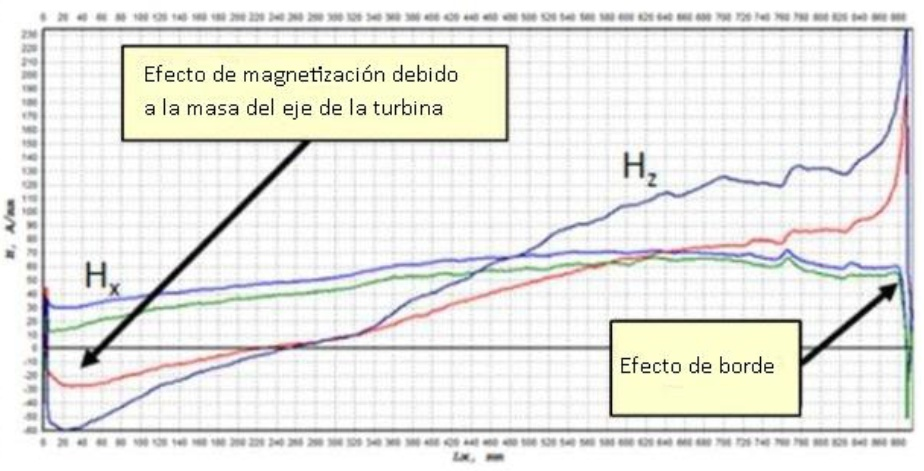
\includegraphics[width=0.8\textwidth]{./Figures/fig53}
	\caption{Campos soble el canto del álabe}
	\label{fig:53}
\end{figure}

Cuando el material es sometido a esfuerzos se observa una ariación de la magnetización en función de la tensiones inducidas en el sólido. Ver figura \ref{fig:54}. Este fenómeno es todavía mucho más marcado en materiales compuestos como las ferritas 

\begin{figure}[H]
    \centering
    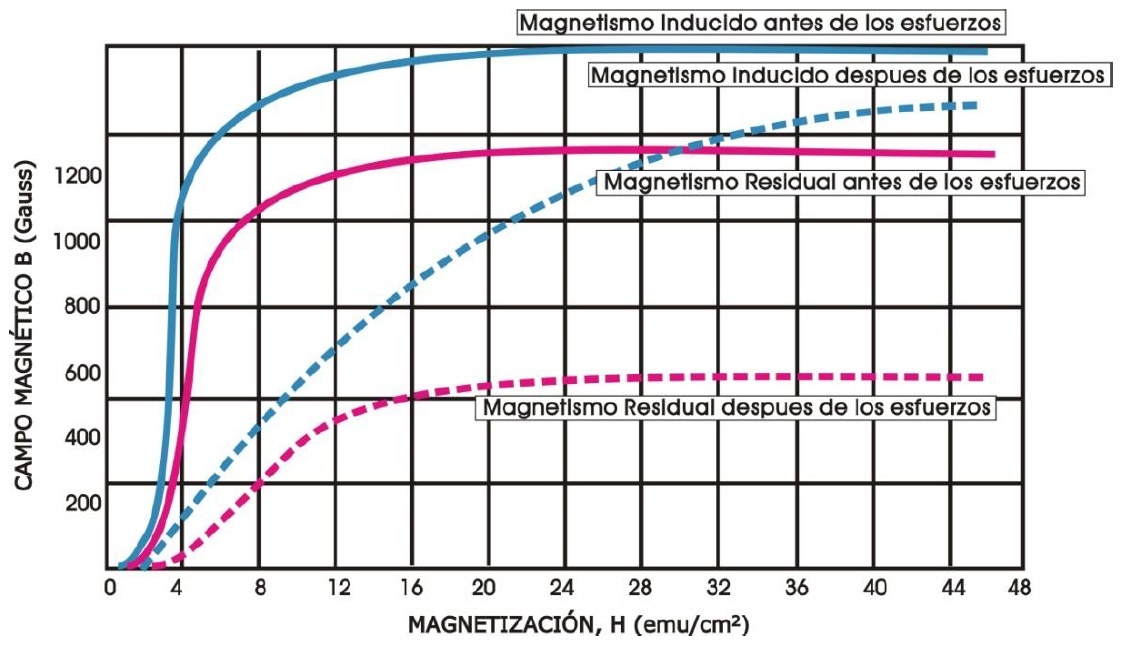
\includegraphics[width=1.0\textwidth]{./Figures/fig54}
	\caption{Variación de la magnetización por tensiones inducidas}
	\label{fig:55}
\end{figure}


Asimismo se observa también una variación de la magnetización en función del número de ciclos de trabajo (tensiones). como ejemplo tenemos la figura \ref{fig:55} donde se observa la variación de la magnetización para distintos esfuerzos longitudinales en mechas de acero de un mismo lote.

\begin{figure}[H]
    \centering
    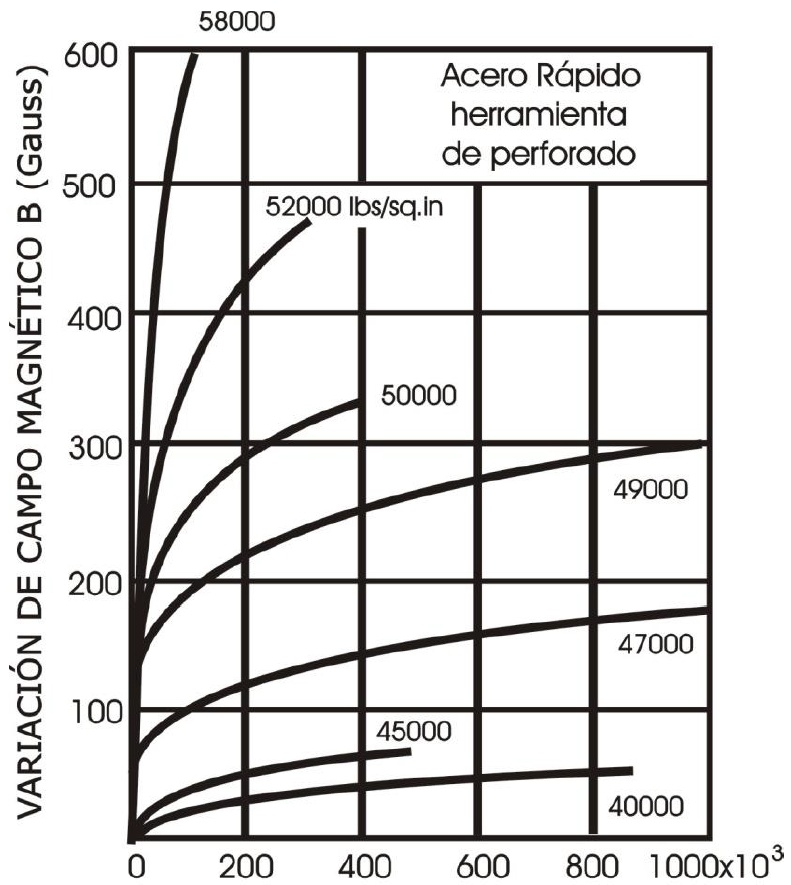
\includegraphics[width=0.6\textwidth]{./Figures/fig55}
	\caption{Variación de magnetización en mechas de acero}
	\label{fig:55}
\end{figure}


\subsection{Caracterización multipolar de una anomalía magnética localizada.}
En el aire la inducción $\vec{B}$ y la excitación $\vec{H}$ son proporcionales: $\vec{B} = \mu_{0}\vec{H}$. En el medio sólido sabemos que: $\vec{B} = \mu_{0}\vec{H} + \vec{M}\;$, siendo $\vec{M}$ la Magnetización\footnote{\url{https://en.wikipedia.org/wiki/Magnetization}}. 

En el caso de ausencia de corrientes podremos plantear que $\vec{\nabla}\times\vec{H} = 0$ y como siempre $\vec{\nabla}\cdot\vec{B} = 0$, entonces resultará que:
\begin{equation}
	\label{eq:mediosLIH6}
	\vec{\nabla}\cdot\vec{H} = -\dfrac{1}{\mu_{0}}\vec{\nabla}\cdot\vec{M}
\end{equation}
Por lo tanto podremos poner que $\vec{H} = -\vec{\nabla}\varphi_{M}$ siendo $\varphi_{M}(\vec{r})$ un potencial escalar magnético que verifica la ecuación de Poisson:

\begin{equation}
	\label{eq:Poisson}
	\nabla^2\varphi_{M}(\vec{r}) = \dfrac{1}{\mu_{0}} \nabla \cdot\vec{M}(\vec{r}) 
\end{equation}

La ecuación de Poisson \ref{eq:Poisson} se puede resolver por el método de Gauss-Green \citep{GaussGreen} y la solución resulta de la forma:

\begin{equation}
	\label{eq:GaussGreen}
	\varphi_{M}(\vec{r}) = \dfrac{1}{4\pi\mu_{0}}\iiint_C \dfrac{\rho_{M}(\vec{r'})}{\mid\vec{r}-\vec{r'}\mid} \cdot \,dV' + 
	\dfrac{1}{4\pi\mu_{0}}\iint_{\partial C} \dfrac{\sigma_{M}(\vec{r'})}{\mid\vec{r}-\vec{r'}\mid} \cdot \,dS'
\end{equation}

Donde la integración se lleva a cabo sobre las componentes primadas $\vec{r'}$ para todo el volumen del sólido  $C$ y su frontera ${\partial C}$ siendo $\rho_{M}$ la densidad volumétrica de magnetización y $\sigma_{M}$ la densidad superficial de magnetización

Como solo nos interesan los apartamientos del campo original del sólido sin anomalías, podemos hacer un desarrollo perturbativo\citep{PerturbationMethod}\citep{SingularPerturbation} de la ecuación \ref{eq:Poisson}:



\begin{equation}
	\label{eq:PoissonPerturbada}
	\nabla^2\delta\varphi_{M}(\vec{r}) = \dfrac{1}{\mu_{0}} \nabla \cdot\vec{\delta M}(\vec{r}) 
\end{equation}

Dando su solución un desarrollo análogo al de la ecuación \ref{eq:GaussGreen} con los reemplazos correspondientes de:

\begin{equation}
	\label{eq:GaussGreenReemplazos}
	\rho_{M}   \rightarrow \delta\rho_{M},\;\;
	\sigma_{M} \rightarrow \delta\rho_{M},\;\;	  
	C \rightarrow R_{mag}, \;\;	  
	\partial C \rightarrow \partial C \cap R_{mag} = \partial R_{mag}
\end{equation}

Notemos que podrá ser la frontera $\partial C \cap R_{mag}$ vacía si la región de influencia de los defectos significativos no llega hasta la superficie del sólido y el término con $\partial R_{mag}$ desaparecer de \ref{eq:GaussGreen}. Por el contrario si el defecto es justamente una discontinuidad en la superficie del sólido como el indicado en la figura \ref{fig:MMM_dispersion} el vacío sera el conjunto $R_{mag}$ y solo aportara al campo su frontera $\partial R_{mag}$

En el aire próximo a la superficie de la pieza, la perturbación $\delta\rho_{M}$ se puede expresar mediante un desarrollo multipolar respecto de un origen de coordenadas localizado en el interior del defecto $R_{mag}$, de modo que el vector posición $\vec{r}$ del punto donde se considera el campo posea un módulo $r$ mayor que el de cualquier vector posición $\vec{r'}$ correspondientes a los puntos donde $\delta \vec{M}(\vec{r'}) \neq 0$. La expresión del desarrollo multipolar correspondiente quedará como:

\begin{equation}
	\label{eq:DesarrolloMultipolar}
	\delta\varphi_{M} \approx \delta\varphi_{M dipolar} + \delta\varphi_{M cuadrupolar} + . . . + . . . 
\end{equation}

Puesto que no existen monopolos magnéticos el desarrollo comenzará con el término dipolar $\delta\vec{\lambda}$ caracterizado por tres componentes de momento dipolar independientes:

\begin{equation}
	\label{eq:Dipolo}
	\delta\vec{\lambda} = \iiint_{R_{mag}} \delta\rho_{M}\; \vec{r'} \,dV' + 
	\iint_{\partial R_{mag}} \delta\sigma_{M}\;  \vec{r'} \,dS'
\end{equation}

Siendo el término correspondiente en el desarrollo multipolar: 

\begin{equation}
	\label{eq:GaussGreenDipolo}
	\delta\varphi_{M}(\vec{r})_{dipolar} \approx \dfrac{1}{4\pi\mu_{0}} \dfrac{\delta\vec{\lambda} \cdot \vec{r}}{r^3}
	, \;\;\;\; \mid \vec{r} \mid \gg \mid \vec{r'} \mid 
\end{equation}



El siguiente término, correspondiente al momento cuadrupolar viene caracterizado por cinco coeficientes de cuadrupolo independientes:

\begin{equation}
	\label{eq:Cuadrupolo}
	\delta Q_{ij} = \iiint_{R_{mag}} \delta\rho_{M}\;  \left( 3 x'_{i}x'_{j}-r'^2 \delta_{ij} \right) \,dV' + 
	\iint_{\partial R_{mag}} \delta\sigma_{M}\;  \left( 3 x'_{i}x'_{j}-r'^2 \delta_{ij} \right) \,dS'
\end{equation}

donde $\delta_{ij}$ representa la función delta de Kronecker \footnote{\url{https://en.wikipedia.org/wiki/Kronecker\_delta}}. Observemos que aunque $\delta Q_{ij}$ tiene nueve componentes de su definición resulta que es simétrico y de traza nula \textit{i.e.} $Q_{kl}=Q_{lk}$ y $Q_{11}+Q_{22}+Q_{33}=0 $ razones éstas por lo que solo habrá cinco componentes independientes.

Quedando el término correspondiente en el desarrollo multipolar: 

\begin{equation}
	\label{eq:GaussGreenCuadrupolo}
	\delta\varphi_{M}(\vec{r})_{cuadrupolo} \approx 
	\dfrac{1}{4\pi\mu_{0}} 
	\dfrac{\vec{r} \cdot \delta\hat{Q} \cdot \vec{r}}{r^5}
\end{equation}

Fuera del sólido los términos cuadrupolares, octpolares y demás siguientes en la serie tienen  un rápido decaimiento debido a la fuerte dependencia con $\dfrac{1}{r^{2n+1}}$ para $n \geq 3, 4, ... $. siendo su aporte al campo $\delta\vec{H}$ de segundo orden con respecto al del dipolo. Por lo tanto considerando la perturbación a primer orden, sólo serán relevantes los términos dipolares. Recordemos que estamos hablando de la perturbación $\delta\vec{H}$ y no del campo base $\vec{H}$.     

Tendremos entonces que: la perturbación $\delta\vec{H}$ a primer orden del campo excitación $\vec{H}$ en las proximidades de la superficie del sólido debido a la presencia de un defecto en la región $R_{mag}$ será:

\begin{equation}
	\label{eq:GaussGreenFinal}
	\delta\vec{H}(\vec{r}) = -\nabla\delta\varphi_{M} \approx \dfrac{1}{4\pi\mu_{0}}\left(  
	\dfrac{-\delta\vec{\lambda}}{{\mid\vec{r}-\vec{r_{d}}\mid}^3} + 
	\dfrac{	\left( \delta\vec{\lambda} \cdot \left( \vec{r}-\vec{r_{d}} \right) \right) }{ {\mid\vec{r}-\vec{r_{d}}\mid}^5} 
	\left( \vec{r}-\vec{r_{d}} \right) \right) 
\end{equation}


Siendo $\vec{r_{d}}$ la posición del dipolo $\vec{\lambda}$ respecto de un origen externo de coordenadas fijado arbitrariamente .

A partir de mediciones de $\delta\vec{H}(\vec{r_{k}}) $ se pueden estimar la posición $\vec{r_{d}}$ y las componentes de $\delta\vec\lambda$ aplicando modelos de regresión no lineal\citep{EstimacionNoLineal1}, pudiendo emplearse el algoritmo de Gauss-Newton\footnote{\url{https://en.wikipedia.org/wiki/Gauss-Newton\_algorithm}} cuando se trata de defectos bien localizados como en el caso de fisuras superficiales o próximas a la superficie del sólido . 


De ser necesario continuar a segundo orden con las componentes del desarrollo cuadrupolar, luego de determinarse $\vec{r_{d}}$ y $\delta\vec\lambda$ éstas se eliminarían como incógnitas de la ecuación \ref{eq:GaussGreenFinal} y se le sumaría el término correspondiente al cuadrupolo: 

\begin{equation}
	\label{eq:GaussGreenCuadrupoloFinal}
	-\nabla\delta\varphi_{M}(\vec{r})_{cuadrupolo} \approx 
	-\nabla \left( \dfrac{1}{4\pi\mu_{0}} 
	\dfrac{\vec{r} \cdot \delta\hat{Q} \cdot \vec{r}}{r^5}\right) 
\end{equation}

Los cinco coeficientes cuadrupolares incógnita ahora podrán calcularse tomando una nueva serie de mediciones $\delta\vec{H}(\vec(r_{k}) $ y aplicando nuevamente un modelo de regresión no lineal. Para esta forma de funciones en particular resulta apropiado el modelo de Levenberg-Marquardt \citep{EstimacionNoLineal2}. éste modelo es más robusto que el de Gauss-Newton y resulta muy útil cuando no se tiene bien establecida una zona de confianza\footnote{\url{https://en.wikipedia.org/wiki/Levenberg-Marquardt\_algorithm}}.


\subsubsection{Termodinámica de la anomalía localizada}

El análisis termodinámico detallado del potencial Gibbs magnetoelástico y sus variantes, con las energías involucradas en las tensiones y los potenciales termodinámicos involucrados con los términos de magneto estricción y magneto elasticidad permite hallar una relación entre las tensiones y la permeabilidad aparente de material:

\begin{equation}
	\label{eq:522}
	du = T \cdot dS + \bar{\bar{\sigma}} \cdot d\bar{\bar{\varepsilon}} + \overrightarrow{H} \cdot d \overrightarrow{B}
\end{equation}

Aplicando la transformación de Legendre:

\begin{equation}
	\label{eq:523}
	g = u - T \cdot S  + \bar{\bar{\sigma}} \cdot \bar{\bar{\varepsilon}}  + \overrightarrow{H} \cdot \overrightarrow{B}
\end{equation}

Resulta:

\begin{equation}
	\label{eq:524}
	dg = - S \cdot dT  - \bar{\bar{\varepsilon}} \cdot d\bar{\bar{\sigma}} - \overrightarrow{B} \cdot d\overrightarrow{H}
\end{equation}

Con lo que se verifica que:

\begin{equation}
	\label{eq:525}
	B_{i}=\left(\dfrac{\partial g}{\partial H_{i}} \right)_{T,\bar{\bar{\sigma}}} \, , \,
	\bar{\bar{\epsilon}}=\left(\dfrac{\partial g}{\partial \bar{\bar{\sigma}}} \right)_{T,\overrightarrow{H}} \, , \,
\left(\dfrac{\partial \epsilon}{\partial H_{i}} \right)_{T,\bar{\bar{\sigma}}} = 
\left(\dfrac{\partial B_{k}}{\partial \bar{\bar{\sigma}}} \right)_{T,\overrightarrow{H}}
\end{equation}
	 
Donde vemos los coeficientes de magnetostricción: $\left(\dfrac{\partial \epsilon}{\partial H_{i}} \right)_{T,\bar{\bar{\sigma}}}$ y de magnetoelasticidad: $\left(\dfrac{\partial B_{k}}{\partial \bar{\bar{\sigma}}} \right)_{T,\overrightarrow{H}}$.

Debemos notar también que:	

\begin{equation}
	\label{eq:526}
\left(\dfrac{\partial B_{k}}{\partial \bar{\bar{\sigma}}} \right)_{T,\overrightarrow{H}}=
\left(\dfrac{\partial M_{k}}{\partial \bar{\bar{\sigma}}} \right)_{T,\overrightarrow{H}}
\end{equation}

Puesto que $B_{k}=\mu_{0}H_{k}+M_{k}$, si el campo $H$ permanece constante entonces será $B=M$

Plantendo y despejando $\mu=\mu_{0} \mu_{r} = \dfrac{B}{H} $ , luego de varias cuentas, linearizaciones y asunciones, tenemos que:

\begin{equation}
	\label{eq:527}
	\mu= \dfrac{1}{(\beta-q\sigma-R\sigma^{2})+\dfrac{K_{0}}{12}B^{2}+\dfrac{K_{1}}{90}B^{4}}
\end{equation}

Donde $\sigma=\bar{\bar{\sigma}}$ es el tensor de tensiones, $q=q_{i,j,k,l}$ los parámetros de magnetoelasticidad, $R=R_{i,j,k,l}$ los denominados coeficientes de corrección mórfica de las complacencias elásticas (que tienen en cuenta el efecto del campo $B$ sobre los módulos de elasticidad y $\beta=\bar{\bar{\beta}}$, $K_{0}={K_{0}}_{i,j,k,l}$, $K_{1}={K_{1}}_{i,j,k,l,m,n}$ son parámetros de “impermeabilidad magnética” que describen la relación entre $H$ y $B$ cuando los esfuerzos mecánicos son nulos y por ende no hay efecto magneto-elástico.

Esta relación vincula en forma completamente general los efectos magneto-estrictivo y magneto-elástico y estima la influencia del estado local de tensiones mecánicas sobre la permeabilidad magnética local del material.

\textbf{Una consecuencia inmediata es que una heterogeneidad magnética primaria (cavidad o inclusión no ferromagnética) podría comportarse en forma no distinguible de una heterogeneidad magnética secundaria (concentración de tensiones) cuando la única información disponible proviene de la medición del auto-campo de fuga en el aire próximo a la superficie de la pieza}.


En la figura \ref{fig:56} vemos los campos resultantes del escaneo magnético en tres ejes a 2 mm de la superficie de una chapa de acero soldada a tope con otra, tomado a lo largo de la soldadura. El eje z es vertical a la soldadura, el eje x a lo largo y el eje y transversal.
Se pueden observar diversas zonas con tensiones como las indicadas en las figura 1. complemetarias en los ejes x y z. La inspección visual no revela en la soldadura fisuras superficiales.

\begin{figure}[H]
    \centering
    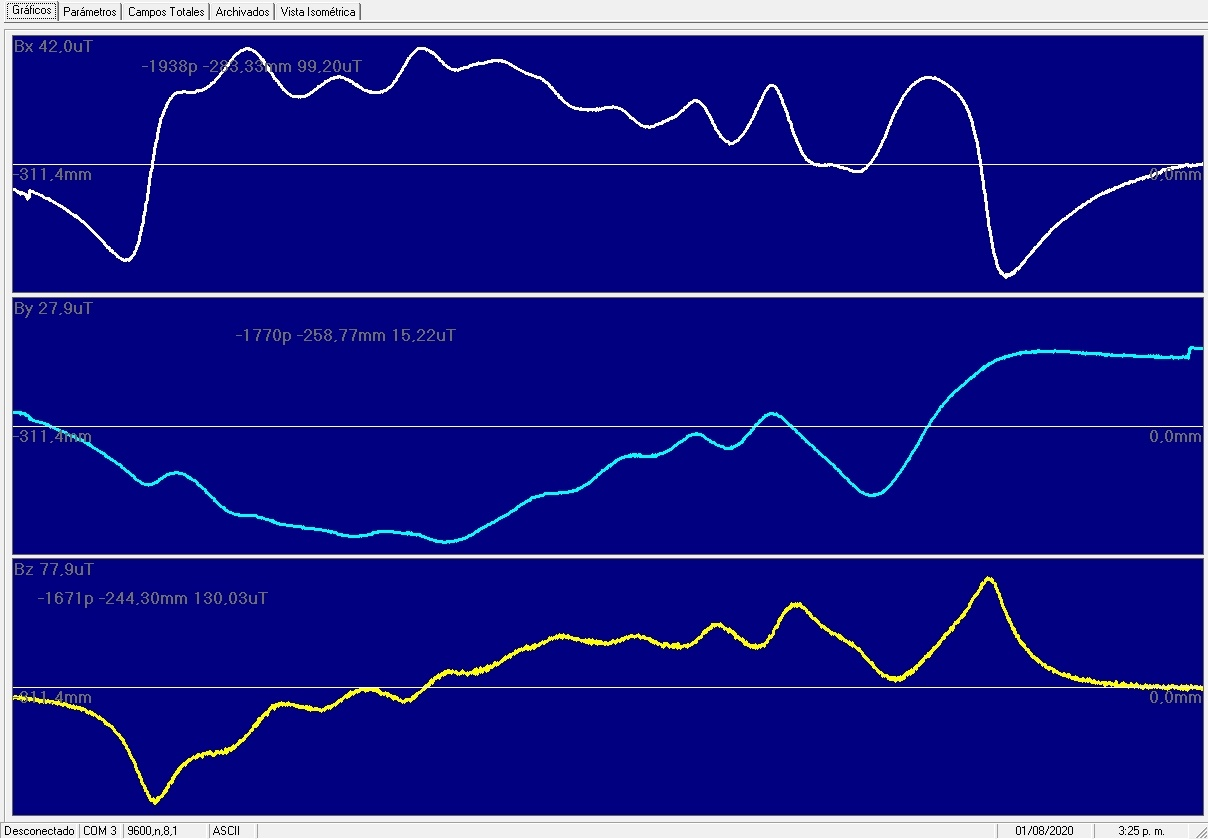
\includegraphics[width=1.0\textwidth]{./Figures/fig56b}
	\caption{Campos en los ejes $x$, $y$ y $z$}
	\label{fig:56}
\end{figure}

\section{Sólidos Conductores}

A diferencia de los sólidos ferromagnéticos, los sólidos conductores que no presentan magnetización residual pueden caracterizarse en regiones cercanas a las superficie induciendo en ellos corrientes de Foucault (\textit{Eddy Currents} o corrientes turbillonarias) por medio de una excitación magnética externa y levantando los perfiles de campo producidos por estas corrientes en el material.

La profundidad de penetración (\textit{skin deep}) es la tendencia de una corriente eléctrica alterna (CA) a distribuirse dentro de un conductor de forma exponencial decreciente, de modo que la densidad de corriente sea mayor cerca de la superficie del conductor y disminuya con mayores profundidades en el conductor. La corriente eléctrica fluye principalmente en la "piel" del conductor, entre la superficie exterior y un nivel llamado profundidad de penetración. El efecto del skin deep hace que la resistencia efectiva del conductor aumente a frecuencias más altas donde la profundidad de penetración es menor, reduciendo así la sección transversal efectiva del conductor. Como se ha ya mencionado, el efecto se debe a las corrientes de Foucault opuestas inducidas por el campo magnético cambiante resultante del flujo magnético alterno.

A $60 Hz$ en cobre, la profundidad de la piel es de aproximadamente $8,5 mm$. A altas frecuencias, la profundidad de penetración se vuelve consecuentemente más pequeña según la ley:

\begin{equation}
	\label{eq:528}
	\delta= \sqrt{\dfrac{2\rho}{\omega\mu}}\sqrt{\sqrt{1+(\rho\omega\epsilon)^{2}}+\rho\omega\epsilon} \, , \, \omega=2\pi f
\end{equation}

Siendo $\delta$ la profundidad de penetración, $\epsilon$ la permitividad del conductor $\mu$ la permeabilidad y $f$ la frecuencia del flujo magnético.

Para la densidad de corriente tendremos que:

\begin{equation}
	\label{eq:529}
	J=J_{0}e^{-(1+i)\dfrac{d}{\delta}}
\end{equation}

Lo que nos dice que a una profundidad de $\delta$ tendremos una disminución proporcional de $e^{-1}$ en la intensidad de la corriente (lo que es aproximadamente un 67\%)

De todo lo anterior podemos ver que ajustando la frecuencia podemos extraer información de los defectos del material a distintas profundidades. En oposición a esto tenemos que al aumentar la profundidad y disminuir la frecuencia, para un mismo flujo dado, la corriente neta disminuye proporcionalmente produciendo señales de campos inducidos más débiles.

En función de la conductividad del material es de esperarse que la profundidad de penetración (\textit{skin deep}) sea solo función de la frecuencia del campo inducido a frecuencias bajas donde la masa de los electrones sea despreciable.

El caso general de las corrientes inducidas ha sido estudiado en detalle y tienen muchas aplicaciones, entre ellas:


\begin{itemize}
	\item Discontinuidades en material conductor tales como cambios geométricos, variación de las propiedades relacionadas con la conductividad y permeabilidad.
	
	\item Presencia de defectos, tanto superficiales como subterráneas, detección de defectos y grieta en el material de soldadura conductivo.
	
	\item Detectar de corrosión, daño por fatiga y adelgazamiento. En particular, la técnica se usa para hacer mediciones de corrosión y adelgazamiento en material aeronáutico e intercambiadores de calor.
	
	\item La permeabilidad y la conductividad son los factores que más afectan la señal, por lo que las corrientes parásitas se pueden usar para distinguir entre diversos tipos de materiales y para
determinar si un material ha sido expuesto a altas temperaturas, en los casos en que dichos tratamientos cambien el conductividad del material.

\end{itemize}

En las circunstancias adecuadas, las corrientes parásitas se pueden usar para:

\begin{itemize}
	\item Detección de grietas.
	\item Mediciones de espesor de material.
	\item Medidas de espesor de recubrimiento.
	\item Mediciones de conductividad para:
	\begin{itemize}
		\item{a} Identificación del material
		\item{b} Detección de daños por calor
		\item{c} Determinación de profundidad
		\item{d} Monitoreo de tratamiento térmico
	\end{itemize}	
\end{itemize}

Algunas de las ventajas de la inspección por corrientes de Foucault incluyen:

\begin{itemize}
	\item Sensibilidad a pequeñas grietas y otros defectos.
	\item Detección defectos superficiales y cercanos a la superficie.
	\item La inspección da resultados inmediatos.
	\item El equipo es muy portátil.
	\item El método puede usarse para otras aplicaciones.
	\item Se requiere una preparación mínima.
	\item La sonda de prueba no necesita ponerse en contacto con la pieza.
	\item Inspecciona formas y tamaños complejos de materiales conductores.
\end{itemize}

Algunas de las limitaciones de la inspección por corrientes de Foucault incluyen:

\begin{itemize}
	\item Solo se pueden inspeccionar materiales conductores.
	\item La superficie debe ser accesible para la sonda.
	\item La habilidad y capacitación requerida es más extensa que en otras técnicas.
	\item El acabado superficial y la aspereza pueden interferir.
	\item No hay estándares de referencia necesarios para la configuración.
	\item La profundidad de penetración es limitada.
	\item Los defectos como los de laminaciones que se encuentran paralelas al devanado de la bobina de la sonda y la dirección de exploración de la sonda son indetectables.
\end{itemize}

\subsection{Método de las Corrientes Parásitas ECM}

El método de las corriente parásita o ECM (\textit{Eddy Current Method}) consiste en aproximar una bobina excitadora que genera un campo magnético armónico sinusoidal en el rango de los Hz hasta los MHz, producido por una corriente senoidal. Las variaciones de flujo del campo magnético en el material induce corrientes parásitas en la zona bajo examen. Ante estas corrientes la presencia de defectos o discontinuidades se comportan como una barrera resistiva que perturba los flujos de corriente inducidos. Las perturbaciones resultantes afectan los campos magnéticos superficiales, permitiendo detectar las anomalías.

En la figura \ref{fig:57} vemos los campos en un sustrato normal, con conductividad uniforme y en un sustrato con un defecto resistivo.

\begin{figure}[H]
    \centering
    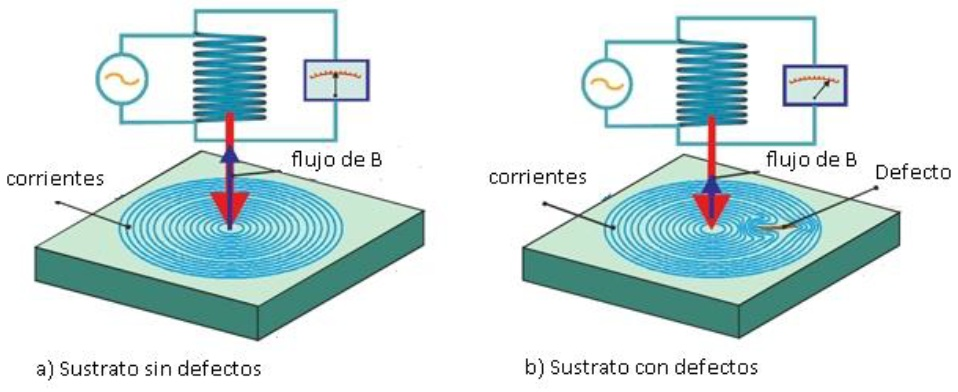
\includegraphics[width=1.0\textwidth]{./Figures/fig57}
	\caption{Corrientes turbillonarias en diversos sustratos}
	\label{fig:57}
\end{figure}

Si el material fuera un conductor perfecto, los campos magnéticos producidos por las corrientes turbillonarias se verían como si se estuviera hubiera en presencia de un inductor igual al impuesto en la excitación dispuesto en forma espejada respecto de la superficie del otro lado de material, esto se conoce como espejo de corrientes y en el caso de una excitación con alta simetría frente a una superficie plana o de curvatura regular, el campo resultante es fácilmente relevable en busca de imperfecciones.

Las fórmulas de Maxwell y constitutivas del medio aplicables al método son:

\begin{equation*}
	\label{eq:530}
	\nabla \times H= J + \dfrac{\partial E}{\partial t}, \quad
	\nabla \times H= - \dfrac{\partial B}{\partial t}, \quad	
	\nabla \cdot  B= 0, \quad
	\nabla \cdot  E= 0
\end{equation*}
\begin{equation*}
	\label{eq:531}
	B=\mu H \quad	\text{y} \quad J=\sigma E
\end{equation*}

La solución \textbf{práctica} al problema de la distribución de campo en la superficie sigue el mismo principio general ya expresado de considerar la influencia de los defectos con el método perturbativo. El campo base se calcula por el método de las imágenes ya descripto anteriormente y a este se añade el campo de la perturbación que debe cumplir con las condiciones de frontera del sólido.

La solución \textbf{general} a los campos se puede plantear en términos de ecuaciones integrales de la forma:

\begin{equation}
	\label{eq:532}
	H_{ext} = H_{0}+\int_{Sup}\left[J_{S}\times\nabla G_{0}-\dfrac{\nabla_{s}\cdot K_{s}}{i\omega\mu_{0}} \nabla G_{0} \right]dS 
\end{equation}

\begin{equation}
	\label{eq:533}
	E_{ext} = E_{0}+\int_{Sup}\left[i\omega\mu_{0}J_{S}G_{0}+K_{S}\times \nabla G_{0}-\dfrac{\nabla_{s}\cdot J_{s}}{i\omega\epsilon_{0}} \nabla G_{0} \right]dS 
\end{equation}

\begin{equation}
	\label{eq:534}
	H_{int} = -\int_{Sup}\left[\sigma K_{S} G_{i}+ J_{S} \times \nabla G_{i}-\dfrac{\nabla_{s}\cdot K_{s}}{i\omega\mu_{i}} \nabla G_{i} \right]dS 
\end{equation}

\begin{equation}
	\label{eq:535}
	E_{int} = \int_{Sup}\left[i\omega\mu_{i}J_{S}G_{i}+K_{S}\times \nabla G_{i} \right]dS 
\end{equation}

Los términos $H_{0}$ y $E_{0}$ son los campos excitadores en ausencia del medio conductor y $G_{i}$ y $G_{0}$ son las funciones de Green:

\begin{equation*}
	\label{eq:536}
	G_{0}=\dfrac{e^{-i\omega \overrightarrow{K_{0}}\cdot \overrightarrow{r}}}{4\pi r}, \quad
	G_{i}=\dfrac{e^{-i\omega \overrightarrow{K_{i}}\cdot \overrightarrow{r}}}{4\pi r}, \quad	
	K_{0}=\sqrt{\mu_{0}\epsilon_{0}}, \quad
	K_{i}=\sqrt{\mu_{i}\sigma}
\end{equation*}


\subsection{Configuraciones de medición}

Es posible adoptar dos configuraciones de medición para el método de las corrientes parásitas:

\begin{itemize}
	\item \textbf{Excitación y sensor en la misma bobina}: Se mite tensión y fase sobre la bobina excitadora y se representan las variaciones de impedancia en un plano x, Z . Tiene la ventaja de que el dispositivo es muy sencillo, pues la misma bobina excitadora es la que releva el campo de las corrientes inducidas. Sin embargo, solo se puede medir en el mismo punto donde se coloca la bobina excitadora, limitando el alcance a las regiones donde cabe esta.
	
	\item \textbf{Sensor independiente de la excitación}: Se miden los campos magnéticos independientemente de la excitación con un sensor aparte. Tiene la ventaja de la versatilidad y de poder explorar regiones a distintas distancias de la bobina excitadora pues los sensores magnéticos pueden tener dimensiones milimétricas. Este método tiene además la gran ventaja de que perfilando el área de la bobina sensora es posible efectuar un filtrado de las componentes multipolares por cuanto el alcance relativo de cada componente es proporcional al área y a la distancia a la superficie.
\end{itemize}

\subsubsection{Excitación y sensor en la misma bobina}

En la figura \ref{fig:58a} vemos la lobina excitadora usada también como sensor. Las variaciones de tensión y corriente en la bobina dependen tanto de su propia excitación como del flujo inducido por las corrientes superficiales. 

\begin{figure}[H]
    \centering
    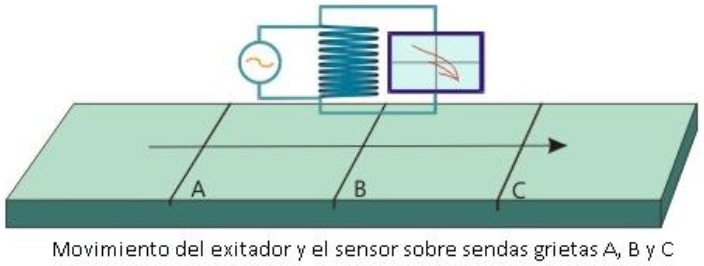
\includegraphics[width=0.8\textwidth]{./Figures/fig58a}
	\caption{Exitación y sensor en la misma bobina}
	\label{fig:58a}
\end{figure}

En la figura \ref{fig:58b} vemos la gráfica de la impedancia equivalente vista por la excitación de la primaria de la bobina en sus componente resistiva e inductiva, dando evidencia de la presencia de grietas a medida que avanza.

\begin{figure}[H]
    \centering
    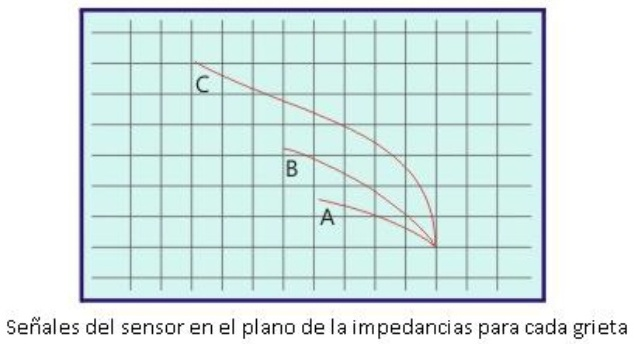
\includegraphics[width=0.8\textwidth]{./Figures/fig58b}
	\caption{Relación de las impedancias en presencia de una grieta}
	\label{fig:58b}
\end{figure}

En la figura \ref{fig:59} vemos un equipo comercial explorando una pieza mecánica. La presencia de grietas se pone en evidencia por los apartamientos de la linealidad que se observan en la pantalla de la derecha

\begin{figure}[H]
    \centering
    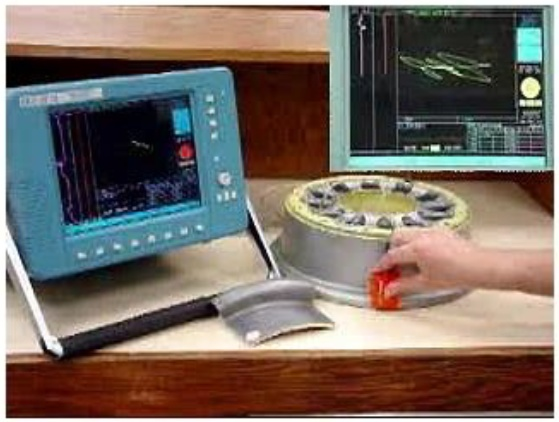
\includegraphics[width=0.7\textwidth]{./Figures/fig59}
	\caption{Graficos de impedancias}
	\label{fig:59}
\end{figure}


\subsubsection{Sensor independiente de la excitación}


En la figura \ref{fig:510} vemos la disposición de una bobina excitadora independiente del sensor. Para simplificar el método de imágenes magnéticas en el medio conductor, la bobina exitadora consiste en conductores planos rectos paralelos a la superficie a explorar. El sensor son otras bobina donde las distintas geometrías posibles, permiten discriminar los aportes multipolares de la distribución de corrientes.

\begin{figure}[H]
    \centering
    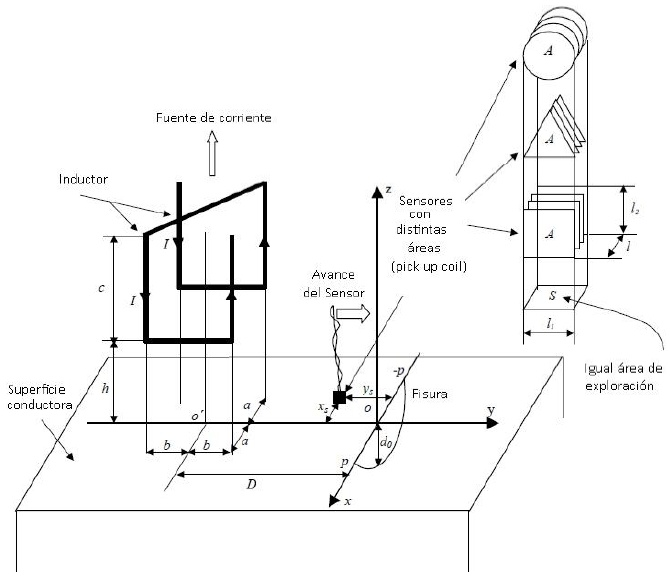
\includegraphics[width=1.0\textwidth]{./Figures/fig510}
	\caption{Distintos perfiles de bobinas}
	\label{fig:510}
\end{figure}

La salida de tensión en la bobina sensora se puede obtener por la lay de Faraday:

\begin{equation}
	\label{eq:537}
	v(x,y) = -\dfrac{d\varphi_{tot}}{dt}=-\int_{l}\dfrac{\varphi_{l}}{dt}dx=-i\omega\int_{l}dx\iint_{A}B_{x}(x,y)dxdy
\end{equation}

Siendo $l$ cada espira individual de la bobina, $\varphi_{tot}$ el flujo total, $\varphi_{l}$ el flujo individual por la espira l-ésima y en la última igualdad hemos asumido que se trata de una excitación sinusoidal para eliminar la derivada temporal. La variación en $B_{x}$ en la dirección $z$ se asume despreciable.

Conocido el perfil de la espira $G(x,y)$ podemos reescribir la ecuación \ref{eq:537} como:

\begin{equation}
	\label{eq:537}
	v(0,0) = -i\omega\iint_{A}G(x,y)B_{x}(x,y)dxdy
\end{equation}

Donde los perfiles serian:

Para una espira rectangular de lados $l_{1}$ y $l_{2}$:



\begin{equation}
  G(x,y)=\begin{cases}
  				l_{2}, &\vert x \vert \leqslant \dfrac{l_{2}}{2}; \;  \vert y \vert \leqslant \dfrac{l_{1}}{2}\vspace{0.5cm}\\ 
  				0, &\vert x \vert > \dfrac{l_{2}}{2}; \;  \vert y \vert > \dfrac{l_{1}}{2}
    	\end{cases}
\end{equation}

Para una espira triangular de lados $l_{1}$ y $l_{2}$:

\begin{equation}
  G(x,y)=\begin{cases}
  				l_{2}-2\dfrac{l_{2}}{l_{1}}\vert y \vert, &\vert x \vert \leqslant \dfrac{l_{2}}{2}; \;  \vert y \vert \leqslant \dfrac{l_{1}}{2}\vspace{0.5cm}\\ 
  				\quad \quad 0, &\vert x \vert > \dfrac{l_{2}}{2}; \;  \vert y \vert > \dfrac{l_{1}}{2}
    	\end{cases}
\end{equation}

Para una espira circular simétrica con respecto al plano $z=\dfrac{l_{2}}{2}$ de lados $l_{1}$ y $l_{2}$:

\begin{equation}
  G(x,y)=\begin{cases}
  				\sqrt{l_{1}^{1}-4y^{2}}, &\vert x \vert \leqslant \dfrac{l_{2}}{2}; \;  \vert y \vert \leqslant \dfrac{l_{1}}{2}\vspace{0.5cm}\\ 
  				\quad \quad 0, &\vert x \vert > \dfrac{l_{2}}{2}; \;  \vert y \vert > \dfrac{l_{1}}{2}
    	\end{cases}
\end{equation}


Cuando la bobina sensora se mueve del punto $(0,0)$ al punto $8x_{s}, y_{s})$ tendremos que la tensión será:

\begin{equation}
	\label{eq:538}
	v(x_{s},y_{s}) = -i\omega\iint_{-\infty}^{+\infty}G(x_{s}-x,y_{s}-y)B_{x}(x,y)dxdy
\end{equation}

En otras palabras, la diferencia de tensión entre dos posiciones está relacionada a la convolución de $G(x,y)$ con $B(x,y)$. Ahora podemos usar el Teorema de la Convolución de Fourier:

\begin{equation}
	\label{eq:539}
	Conv\left[ v(k_{x},k_{y})\right] = -i \omega Conv\left[ G(k_{x},k_{y})\right]\cdot Conv\left[ B_{x}(k_{x},k_{y})\right]
\end{equation}

Siendo $k_{x}$, $k_{y}$ las componentes de la frecuencia espacial $k$.

La ecuación \ref{eq:539} indica que la bobina, respecto de la tensión leída a su salida, actúa como un filtro espacial cuyo comportamiento es caracterizado por la función filtro de de la bobina: $G(k)$.

El proceso de deconvolución de la señal se obtiene por medio de algoritmos numéricos que producen los renderizados de la figura \ref{fig:511}. Podemos observar las funciones de perfilado de tres sensores de secciones cuadrada, semicircular y triangular y sus respectivas transferencias de la función filtrado.


\begin{figure}[H]
    \centering
    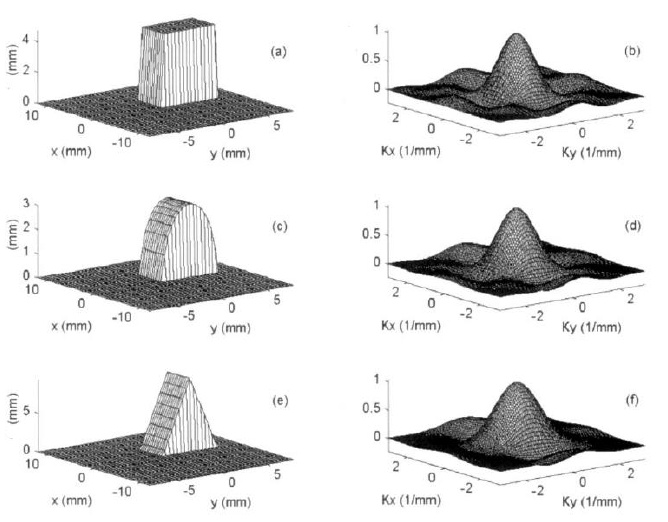
\includegraphics[width=1.0\textwidth]{./Figures/fig511}
	\caption{Efecto de filtro de los distintos perfiles de bobinas}
	\label{fig:511}
\end{figure}

Finalmente, es posible extrapolar la data referida a la señal de la grieta. en la figura \ref{fig:512} tenemos las señales normalizadas de las distintas bobinas sensoras en presencia de una fisura y el resultado de la señal filtrada.

\begin{figure}[H]
    \centering
    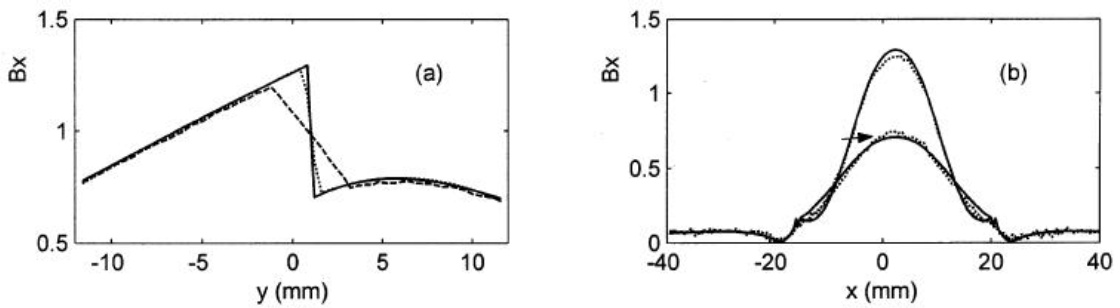
\includegraphics[width=1.0\textwidth]{./Figures/fig512}
	\caption{Señal original y filtrada en proximidad de una fisura}
	\label{fig:512}
\end{figure}








